\documentclass[tikz,border=2mm]{standalone}

\usepackage{amsmath}
\usetikzlibrary{arrows,positioning}
\usetikzlibrary{fit,backgrounds}
\usepackage{xcolor}

\begin{document}

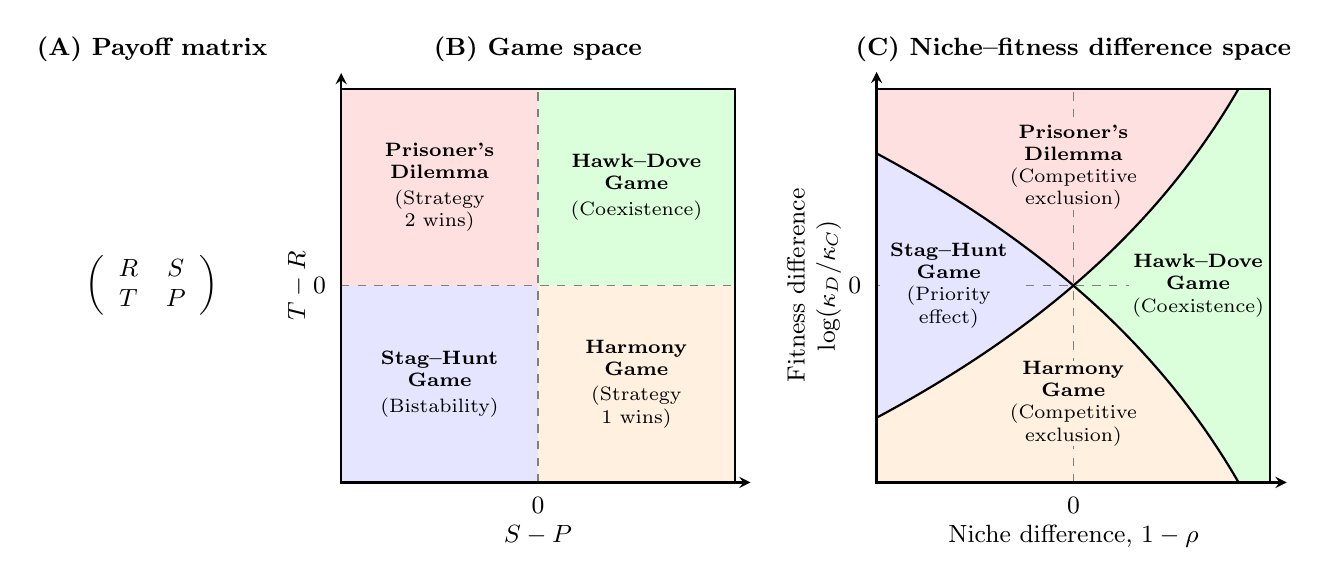
\begin{tikzpicture}[
    >=stealth,
    font=\small,
    gamelabel/.style={
        font=\scriptsize,
        align=center,
        text width=1.75cm,
        inner sep=2pt
    },
    reglabel/.style={
        font=\scriptsize,
        align=center,
        text width=1.75cm,
        inner sep=0pt
    }
]

\colorlet{pdcol}{red!12}
\colorlet{hdcol}{green!14}
\colorlet{shcol}{blue!10}
\colorlet{hmcol}{orange!12}

\node at (-2.7, 3.2) {\textbf{(A) Payoff matrix}};

\node at (-2.7, 0.2) {
    $\left(
    \begin{array}{cc}
    R & S \\
    T & P
    \end{array}
    \right)$
};

\node at (2.2, 3.2) {\textbf{(B) Game space}};

\begin{scope}[shift={(2.2,0.2)}, x=2.5cm, y=2.5cm]
    \def\xmin{-1.0}
    \def\xmax{ 1.0}
    \def\ymin{-1.0}
    \def\ymax{ 1.0}

    \fill[pdcol] (\xmin,0) rectangle (0,\ymax);
    \fill[hdcol] (0,0) rectangle (\xmax,\ymax);
    \fill[shcol] (\xmin,\ymin) rectangle (0,0);
    \fill[hmcol] (0,\ymin) rectangle (\xmax,0);

    \draw[thick] (\xmin,\ymin) rectangle (\xmax,\ymax);

    \draw[dashed, gray] (\xmin,0) -- (\xmax,0);
    \draw[dashed, gray] (0,\ymin) -- (0,\ymax);

    \draw[->, thick] (\xmin,\ymin) -- (\xmax+0.08,\ymin);
    \draw[->, thick] (\xmin,\ymin) -- (\xmin,\ymax+0.08);

    \node[below=12pt] at (0,\ymin) {$S-P$};
    \node[rotate=90] at (\xmin-0.22,0) {$T-R$};

    \node[below=2pt] at (0,\ymin) {$0$};
    \node[left=2pt]  at (\xmin,0) {$0$};

    \node[gamelabel, fill=pdcol] at (-0.5,  0.5)
        {\textbf{Prisoner's}\\\textbf{Dilemma}\\[0.15em](Strategy 2 wins)};

    \node[gamelabel, fill=hdcol] at ( 0.5,  0.5)
        {\textbf{Hawk--Dove}\\\textbf{Game}\\[0.15em](Coexistence)};

    \node[gamelabel, fill=shcol] at (-0.5, -0.5)
        {\textbf{Stag--Hunt}\\\textbf{Game}\\[0.15em](Bistability)};

    \node[gamelabel, fill=hmcol] at ( 0.5, -0.5)
        {\textbf{Harmony}\\\textbf{Game}\\[0.15em](Strategy 1 wins)};
\end{scope}

\node at (9, 3.2) {\textbf{(C) Niche--fitness difference space}};

\begin{scope}[shift={(9,0.2)}, x=4.166667cm, y=3.571429cm]
    \def\xmin{-0.6}
    \def\xmax{ 0.6}
    \def\ymin{-0.7}
    \def\ymax{ 0.7}

    \pgfmathsetmacro{\xcrit}{1 - exp(-\ymax)}

    \begin{scope}
        \clip (\xmin,\ymin) rectangle (\xmax,\ymax);

        \fill[pdcol]
            (\xmin,\ymax) --
            (\xmax,\ymax) --
            plot[domain=\xmax:0, samples=150]
                (\x,{min(-ln(1-\x),\ymax)}) --
            plot[domain=0:\xmin, samples=150]
                (\x,{min( ln(1-\x),\ymax)}) --
            cycle;

        \fill[hmcol]
            (\xmin,\ymin) --
            (\xmax,\ymin) --
            plot[domain=\xmax:0, samples=150]
                (\x,{max( ln(1-\x),\ymin)}) --
            plot[domain=0:\xmin, samples=150]
                (\x,{max(-ln(1-\x),\ymin)}) --
            cycle;

        \fill[shcol]
            plot[domain=\xmin:0, samples=150]
                (\x,{ ln(1-\x)}) --
            plot[domain=0:\xmin, samples=150]
                (\x,{-ln(1-\x)}) --
            cycle;

        \fill[hdcol]
            plot[domain=0:\xmax, samples=150]
                (\x,{max( ln(1-\x),\ymin)}) --
            plot[domain=\xmax:0, samples=150]
                (\x,{min(-ln(1-\x),\ymax)}) --
            cycle;
    \end{scope}

    \draw[thick] (\xmin,\ymin) rectangle (\xmax,\ymax);

    \draw[dashed, gray] (\xmin,0) -- (\xmax,0);
    \draw[dashed, gray] (0,\ymin) -- (0,\ymax);

    \draw[thick]
        plot[domain=\xmin:\xcrit, samples=150]
            (\x,{ ln(1-\x)});

    \draw[thick]
        plot[domain=\xmin:\xcrit, samples=150]
            (\x,{-ln(1-\x)});

    \draw[->, thick] (\xmin,\ymin) -- (\xmax+0.05,\ymin);
    \draw[->, thick] (\xmin,\ymin) -- (\xmin,\ymax+0.06);

    \node[below=12pt] at (0,\ymin)
        {Niche difference, $1-\rho$};

    \node[rotate=90, align=center] at (\xmin-0.19,0)
        {Fitness difference\\$\log(\kappa_D/\kappa_C)$};

    \node[below=2pt] at (0,\ymin) {$0$};
    \node[left=2pt]  at (\xmin,0) {$0$};

    \node[reglabel, fill=pdcol] at (0.00, 0.42)
        {\textbf{Prisoner's}\\\textbf{Dilemma}\\(Competitive exclusion)};

    \node[reglabel, fill=hdcol] at (0.38, 0.00)
        {\textbf{Hawk--Dove}\\\textbf{Game}\\(Coexistence)};

    \node[reglabel, fill=shcol] at (-0.38, 0.00)
        {\textbf{Stag--Hunt}\\\textbf{Game}\\(Priority effect)};

    \node[reglabel, fill=hmcol] at (0.00,-0.42)
        {\textbf{Harmony}\\\textbf{Game}\\(Competitive exclusion)};
\end{scope}

\end{tikzpicture}
\end{document}